\section{Results and Discussion}
System-level simulation was performed with representative AI inference workloads.

\subsection{Standby Power}
Migrating cold data and checkpoints to the FeRAM-backed tier yields more than 30\% reduction in standby power.
This reduction arises from suppressing periodic DRAM refresh for inactive regions.

\subsection{Resume Latency}
FeRAM allows direct restore of checkpoints without full DRAM wake-up.
Resume latency is reduced to the $\mu$s range, enabling near-instant resume after power gating
and improving energy efficiency for mobile edge AI.

\subsection{Endurance}
FeRAM endurance of $10^{12}$ writes/year fits within FeRAM capability for checkpoint traffic.

% ===== Fig.2: Access time vs. Retention (軸レンジと凡例の位置修正) =====
\begin{figure}[t]
\centering
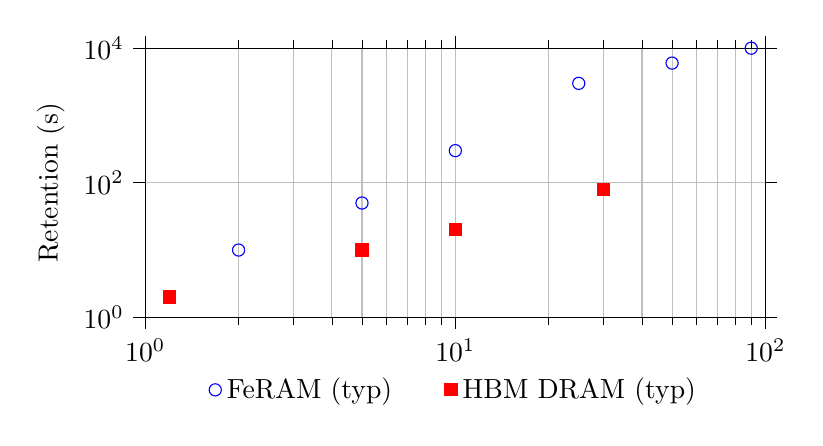
\begin{tikzpicture}
\begin{axis}[
  width=0.78\linewidth, height=5.0cm,
  xmode=log, ymode=log,
  xmin=1, xmax=100, ymin=1, ymax=1e4,
  xlabel={Access time (ns)}, ylabel={Retention (s)},
  grid=both,
  legend columns=2,
  legend style={at={(0.5,-0.18)}, anchor=north, draw=none, /tikz/every even column/.style={column sep=6mm}},
  tick align=outside, tick style={black},
  every axis plot/.append style={only marks, mark size=2.2pt}
]

% --- FeRAM (blue circles) ---
\addplot+[mark=o]
  coordinates {(2,10) (5,50) (10,300) (25,3e3) (50,6e3) (90,1e4)};

% --- HBM DRAM (red squares) ---
\addplot+[mark=square*, mark options={solid}, color=red]
  coordinates {(1.2,2) (5,10) (10,20) (30,80)};

\legend{FeRAM (typ), HBM DRAM (typ)}
\end{axis}
\end{tikzpicture}
\caption{Access time vs.\ retention. Red squares: HBM; blue circles: FeRAM.
Axes are restricted to the practical design window ($10^0\!\sim\!10^2$\,ns, $10^0\!\sim\!10^4$\,s).
The legend is placed \emph{outside} the plot to avoid overlapping points.}
\label{fig:retention_access}
\end{figure}
